\documentclass{beamer}
%
% Choose how your presentation looks.
%
% For more themes, color themes and font themes, see:
% http://deic.uab.es/~iblanes/beamer_gallery/index_by_theme.html
%
\mode<presentation>
{
  \usetheme{default}
  \usecolortheme{default}
  \usefonttheme{default}
  \setbeamertemplate{navigation symbols}{}
  \setbeamertemplate{caption}[numbered]
} 

\usepackage[english]{babel}
\usepackage[utf8]{inputenc}
\usepackage{svg}
\usepackage{amsmath}
\usepackage{listings}
\usepackage{listingsutf8}
\usepackage{listings-golang}
\usepackage{color}
\usepackage{url}

\lstset{ % add your own preferences
    tabsize=2,
    basicstyle=\ttfamily\tiny,
    backgroundcolor=\color{gray!10},
    rulecolor=\color{black!30},
    title=\lstname,
    stringstyle=\color{blue},
    showstringspaces=false, 
    keywordstyle=\color{red},
    frame=single
}

\newcommand\eqdef{\mathrel{\stackrel{\makebox[0pt]{\mbox{\normalfont\tiny def}}}{=}}}

\setbeamertemplate{footline}{\vspace*{1mm}\hfill
\insertframenumber/\inserttotalframenumber\hfill\vspace*{1mm}}



\title{\texorpdfstring{$\pi$\textsf{-calculus and Go}}}
\author{Giorgio Marinelli}
\institute{University of Camerino}
\date{January 21, 2019}



\begin{document}
{ \setbeamertemplate{footline}{}
\begin{frame}[noframenumbering]
  \titlepage
\end{frame}
}


\section{Introduction}
\begin{frame}{Introduction}

\begin{block}{What we are going to do:}
\begin{itemize}
  \item We illustrate and compare the $\pi$-calculus with the Go programming language.
  \item We show how to encode a $\pi$-calculus expression using the Go primitives.
  \item We show, as an example, how to encode the \emph{Church numerals} in the $\pi$-calculus and how they are translated into Go. 
\end{itemize}
\end{block}

\vskip 2em

\begin{block}{\ldots and what we are not going to do}
    We do not show an implementation of the $\pi$-calculus in the Go language, or vice versa.
\end{block}

\end{frame}



\section{The pi-calculus}
\begin{frame}{The $\pi$-calculus}

    The $\pi$-calculus was first presented in ``A Calculus of Mobile Processes'' \cite{Milner89} by Milner, Parrow and Walker in 1989.
    \vskip 1em
    It is an extension of the process algebra CCS.
    \vskip 1em
    It adds the possibility to represent mobile processes, their interconnections evolve during computation.

\end{frame}



\section{The CCS process algebra}
\begin{frame}{The CCS process algebra}

CCS syntax\footnotemark:

\vskip 1em

\begin{center}
$ P ::= \ \  0 \ \  \vert \ \  \alpha.P \ \  \vert \ \  P+Q \ \  \vert \ \  P\vert Q \ \  \vert \ \  P\setminus a $
\end{center}

\vskip 1em

Where: $\alpha$ might be an input channel $a$, an output channel $\bar{a}$, or a silent action $\tau$; $P$ and $Q$ are processes. \\

\vskip 1em

\begin{itemize}
    \item $0$ : the nil process;
    \item $\alpha.P$ : do something and proceed as $P$;
    \item $P+Q$ : act either as P or as Q;
    \item $P\vert Q$ : run $P$ and $Q$ in parallel;
    \item $P\setminus a$ : treat the channel $a$ as private for $P$.
\end{itemize}

\footnotetext[1]{In this CCS syntax, infinite behaviour, relabelling and definitions are not specified.}

\end{frame}


\section{CCS limitations}
\begin{frame}{CCS limitations}

\begin{figure}[t]
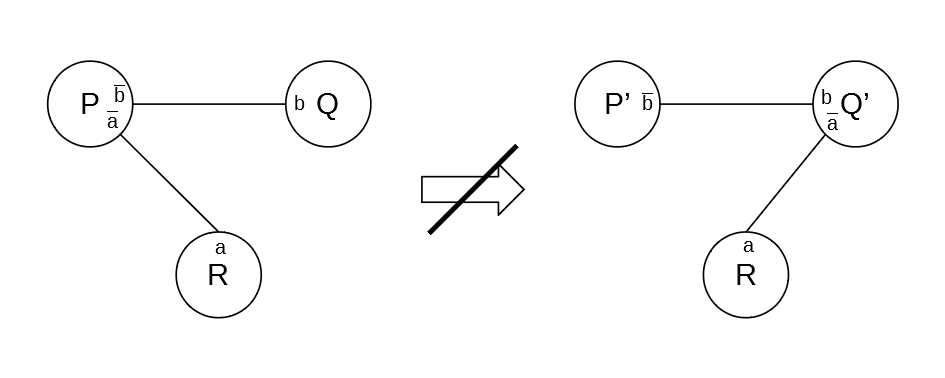
\includegraphics[width=24em]{ccs}
\centering
\caption{Channels as values}
\end{figure}

\vskip 1em

In CCS process algebra this ``transition'' is not possible. The process $P$ should pass the $\bar{b}$ channel to $Q$.

\end{frame}



\section{The pi-calculus syntax}
\begin{frame}{The $\pi$-calculus syntax}

In the $\pi$-calculus we have two primitive entities: \\
names $x,y,\ldots \in \mathcal{X}$ and processes $P,Q,\ldots \in \mathcal{P}$

\vskip 0.2em

Syntax for processes \cite{Milner91}:

\vskip 0.2em

\begin{center}
$ P ::= \ \  \sum_{i \in I} \pi_{i}.P_{i} \ \  \vert \ \  P\vert Q \ \  \vert \ \  !P \ \  \vert \ \  (\nu x)P $
\end{center}

\vskip 0.2em

Where: $\pi_{i}$ might be an input prefix $x(y)$ or an output prefix $\bar{x}y$ . \\

\vskip 0.5em

\begin{itemize}
    \item $\sum_{i \in I} \pi_{i}.P_{i}$ $0$ : act as one of the processes in the sum.\\
    \vspace{0.2em}
    E.g.: with $i=0$, we have the $0$ (or nil) process; with $i=1$, we have $x(y).P$ or $\bar{x}y.P$; with $i=2$, we have $P_{1}+P_{2}$;
    \item $P\vert Q$ : run $P$ and $Q$ in parallel;
    \item $!P$ : replication of $P$, i.e. $P \vert P \vert P \vert \ldots$;
    \item $(\nu x)P$ : ``new $x$ in $P$'', make the name $x$ private for $P$.
\end{itemize}
\end{frame}



\section{The Go programming language}
\begin{frame}{The Go programming language}
    The project was started by Robert Griesemer, Rob Pike and Ken Thompson in 2007.
    \vskip 1em
    In 2009 Go became a public open source project.
    \vskip 1em
    Go has a C-like syntax and concurrency inspired by languages like Newsqueak and Limbo (both of them inspired by Tony Hoare's CSP language).
\end{frame}



\section{The Go syntax}
\begin{frame}[fragile]{The Go syntax}
    Here is a Go program that will print on the screen the string "hello" followed by a number.
    \begin{lstlisting}[language=bash]
$ go run print.go
hello 6
    \end{lstlisting}

    \vskip 0.5em

    \begin{lstlisting}[language=Golang, caption={print.go}, captionpos=b, numbers=left]
package main

import "fmt"

func main() {
	var sum int = 0
	var max int = 4

	for i := 0; i < max; i++ {
		sum += i
	}

	fmt.Println("hello", sum)
}
    \end{lstlisting}
    
\end{frame}



\section{Concurrency in Go}
\begin{frame}[fragile]{Concurrency in Go}
    In Go there are \emph{goroutines}, a sort of lightweight threads, and \emph{channels}, to create communications between \emph{goroutines}.
    \begin{lstlisting}[language=bash]
$ go run channel.go
Run a goroutine
goroutine: 3
main: 5
    \end{lstlisting}
    \begin{lstlisting}[language=Golang, caption={channel.go}, captionpos=b, numbers=left]
package main
import "fmt"

func print_from_channel (channel chan int) {
	var y int = <- channel
	fmt.Println("goroutine:", y)
	channel <- (y + 2)
}

func main () {
	c := make (chan int)
	fmt.Println("Run a goroutine")
	go print_from_channel (c)
	c <- 3
	fmt.Println("main:", <- c)
}
    \end{lstlisting}

\end{frame}



\section{From Pi to Go}
\begin{frame}[fragile]{From $\pi$ to Go}
    Let's see if for every basic process expression of the $\pi$-calculus there exist a corresponding expression or constructor in Go.
    \vskip 1em
\begin{center}
$ P ::= \ \  \sum_{i \in I} \pi_{i}.P_{i} \ \  \vert \ \  P\vert Q \ \  \vert \ \  !P \ \  \vert \ \  (\nu x)P $
\end{center}
    \vskip 1em
    We can consider that any \emph{process} and \emph{name} in the $\pi$-calculus corresponds to a function (or a sequence of statements) and a channel in Go, respectively.
    \vskip 1em

    \begin{lstlisting}[language=Golang, numbers=left]
package main

type Name chan Name

// ...
\end{lstlisting}

\end{frame}



\section{From Pi to Go}
\begin{frame}[fragile]{From $\pi$ to Go : Summation}

    The first $\pi$-calculus expression is $\sum_{i \in I} \pi_{i}.P_{i}$.\\
    We can consider the four basic expressions for the sum:\\

    \begin{itemize}
        \item $0$
        \item $x(y).P$
        \item $\bar{x}y.P$
        \item $P+Q$
    \end{itemize}
\end{frame}



\section{From Pi to Go}
\begin{frame}[fragile]{From $\pi$ to Go : Nil process}

    The $0$ (or \emph{nil}) process might be represented by a function that return anything.

    \begin{lstlisting}[language=Golang, numbers=left]
func nil () {
	return
}
    \end{lstlisting}

\end{frame}



\section{From Pi to Go}
\begin{frame}[fragile]{From $\pi$ to Go : input and output }

    For the input and the output actions we have to use the primitive concurrency operators:
    \vskip 1em
    $x(y).P$ :
    \begin{lstlisting}[language=Golang, numbers=left]
func input_act (x Name, y *Name) {
	*y = <-x
}
    \end{lstlisting}

    \begin{lstlisting}[language=Golang, numbers=left]
x := make (Name)
// ...
var y Name
input_act(x, &y)
P
    \end{lstlisting}

\end{frame}



\section{From Pi to Go}
\begin{frame}[fragile]{From $\pi$ to Go : input and output }

    For the input and the output actions we have to use the primitive concurrency operators:
    \vskip 1em
    $\bar{x}y.P$ :
    \begin{lstlisting}[language=Golang, numbers=left]
func output_act (x Name, y Name) {
	x <- y
}
    \end{lstlisting}

    \begin{lstlisting}[language=Golang, numbers=left]
x := make (Name)
y := make (Name)
// ...
output_act(x, y)
P
    \end{lstlisting}

\end{frame}



\section{From Pi to Go}
\begin{frame}[fragile]{From $\pi$ to Go : $P+Q$}
    The $P+Q$ process behaves as $P$ or $Q$ and the choice is external to this process. We might have, for example:
    \begin{lstlisting}[language=Golang, numbers=left]
func Copy(x, z, y, w Name) {
	select {
	case <- x : Succ (x, z, y, w)      // P process
	case <- z : output_act (w, empty)  // Q process
	}
}
    \end{lstlisting}

\end{frame}



\section{From Pi to Go}
\begin{frame}[fragile]{From $\pi$ to Go : $!P$}
    The $!P$ process could be taught as the repetitive call of the process P. A possibility is to use an infinite loop. For $Q \vert !P$ we could write:
    \vskip 1em
    \begin{lstlisting}[language=Golang, caption={powtwo.go}, captionpos=b, numbers=left]
package main
import "fmt" ; import "math/rand" ; import "time"

func main () {
	x := make (chan int)
	// Q process
	go func (c chan int) { c <- 1 } (x)
	for {
	    // P process
		go func (c chan int) { y := <- c ; fmt.Println(y, " ") ; c <- (y * 2) } (x)
		time.Sleep(time.Duration(100 + rand.Intn(100)) * time.Millisecond)
	}
}
    \end{lstlisting}

    \begin{lstlisting}[language=bash]
$ go run powtwo.go
1 2 4 8 16 32 64 128 256 512 1024 2048 4096 8192 16384 32768 ...
    \end{lstlisting}

\end{frame}



\section{From Pi to Go}
\begin{frame}[fragile]{From $\pi$ to Go : $(\nu x)P$}
    The $(\nu x)P$ process create a new name x and make it private for $P$. We can use the scope a function in Go to create a private channel. E.g.:

    \begin{lstlisting}[language=Golang, numbers=left]
func new() {
    c := make (Name)
    P
}
    \end{lstlisting}

\end{frame}



\section{Church numerals in the pi-calculus}
\begin{frame}{Church numerals in the $\pi$-calculus}
    Church numerals are a way to implement natural numbers in $\lambda$-calculus:
    \vskip 0.5em

    \begin{table}
    \centering
    \begin{tabular}{r|l}
    Natural & Church numeral \\\hline
    0       & $\lambda f . \lambda x . x$ \\
    1       & $\lambda f . \lambda x . f\ x$ \\
    2       & $\lambda f . \lambda x . f (f\ x)$ \\
    3       & $\lambda f . \lambda x . f (f (f\ x))$ \\
    \vdots  & \vdots \\
    n       & $\lambda f . \lambda x . f^{\circ n}\ x$ \\
    \end{tabular}
    \end{table}

    \vskip 0.5em
    Every Church numeral encode the natural number as the number that the function $f$ is applied to its argument $x$.
\end{frame}



\section{Church numerals in the pi-calculus}
\begin{frame}{Church numerals in the $\pi$-calculus}
    In the $\pi$-calculus the computational strategy is different from the ones used in the $\lambda$-calculus. A possible way to implement a natural number $n$ is to encode it with $n$ output prefixes (and an extra output prefix for the zero):
    \vskip 0.5em

    \begin{table}
    \centering
    \begin{tabular}{r|l}
    Natural & \ $\pi$ numeral \\\hline
    0       & $\bar{z}$\footnotemark \\
    1       & $\bar{x} . \bar{z}$ \\
    2       & $\bar{x} . \bar{x} . \bar{z}$ \\
    3       & $\bar{x} . \bar{x} . \bar{x} . \bar{z}$ \\
    \vdots  & \vdots \\
    n       & $(\bar{x}.)^{n} \ \bar{z}$ \\
    \end{tabular}
    \end{table}

    \footnotetext[1]{$\bar{z}$ and $\bar{x}$ are output prefixes where the received name is not associated to any other name like in $\bar{x}y.P$}

\end{frame}



\section{Pi numerals in Go}
\begin{frame}{$\pi$ numerals in Go}
    As presented here \cite{Milner91}, these are the processes for implementing addition between $\pi$ numerals:
    \vskip 1em
    $Add(x_{1} z_{1}, x_{2} z_{2}, y w) \eqdef x_{1}.\bar{y}.Add(x_{1} z_{1}, x_{2} z_{2}, y w) + z_{1}.Copy(x_{2} z_{2})$
    \vskip 1em
    $Copy(x z, y w) \eqdef x.Succ(x z, y w) + z.\bar{w}$
    \vskip 1em
    $Succ(x z, y w) \eqdef \bar{y}.Copy(x z, y w)$
\end{frame}



\section{Pi numerals in Go}
\begin{frame}[fragile]{$\pi$ numerals in Go : $Copy$}
    For the $Copy$ process we have:
    \vskip 1em
    $Copy(x z, y w)  x.Succ(x z, y w) + z.\bar{w}$
    \vskip 1em

    \begin{lstlisting}[language=Golang, numbers=left]
func Copy(x, z, y, w Name) {
	select {
	case <- x : Succ (x, z, y, w)
	case <- z : output_act (w, empty)
	}
}
    \end{lstlisting}
\end{frame}



\section{Pi numerals in Go}
\begin{frame}[fragile]{$\pi$ numerals in Go : $Succ$}
    For the $Succ$ process we have:
    \vskip 1em
    $Succ(x z, y w) \eqdef \bar{y}.Copy(x z, y w)$
    \vskip 1em

    \begin{lstlisting}[language=Golang, numbers=left]
func Succ(x, z, y, w Name) {
	output_act (y, empty)
	Copy (x, z, y, w)
}
    \end{lstlisting}
\end{frame}



\section{Pi numerals in Go}
\begin{frame}[fragile]{$\pi$ numerals in Go : $Add$}
    For the $Add$ process we have:
    \vskip 1em
    $Add(x_{1} z_{1}, x_{2} z_{2}, y w) \eqdef x_{1}.\bar{y}.Add(x_{1} z_{1}, x_{2} z_{2}, y w) + z_{1}.Copy(x_{2} z_{2})$
    \vskip 1em

    \begin{lstlisting}[language=Golang, numbers=left]
func Add(x1, z1, x2, z2, y, w Name) {
	select {
	case <- x1 : output_act (y, empty) ; Add (x1, z1, x2, z2, y, w)
	case <- z1 : Copy (x2, z2, y, w)
	}
}
    \end{lstlisting}
\end{frame}



\section{Pi numerals in Go}
\begin{frame}[fragile]{$\pi$ numerals in Go}

\begin{center}
\vspace*{\fill}
\begingroup
\centering
{\Huge DEMO}
\endgroup
\vspace*{\fill}
\end{center}

\end{frame}



\section{Bibliography}

\begin{frame}{Bibliography}

\begin{thebibliography}{5}
\footnotesize
\setbeamertemplate{bibliography item}[text]
\bibitem{Milner89} Milner, R., Parrow, J.G. and Walker, D.J., \emph{A Calculus of Mobile Processes, Parts I and II}, Report ECS-LFCS-89-85 and -86, Laboratory for Foundations of Computer Science, Computer Science Department, Edinburgh University, 1989.
\bibitem{Milner91} Milner, R., \emph{The Polyadic $\pi$-Calculus: a Tutorial}, Laboratory for Foundations of Computer Science, Computer Science Department, Edinburgh University, 1991.
\bibitem{Marinelli19} Marinelli, G., \emph{pinumerals: Church numerals in the $\pi$-calculus}, University of Camerino, 2019. \url{https://github.com/marinelli/pinumerals}
\end{thebibliography}

\end{frame}



\end{document}
